\chapter{ESDM Implementation}
\label{ch:imp}

\section{Introduction}

ESDM deeply integrates into NetCDF and this chapter describes how ESDM objects are related to NetCDF objects.
For each NetCDF file, ESDM creates a container, and for each NetCDF variable, ESDM creates a dataset.
Listing \ref{esdm-mem} shows the ESDM structures kept in main memory and Listing \ref{esdm-entitites} introduces the ESDM structures kept in disk.

\begin{tcbcode}[label=esdm-mem]{Structures kept in memory by ESDM}
\begin{lstlisting}[upquote=true]
typedef struct {
  int *dimidsp;
  int fillmode; // remembers if fill mode is on or off, by default fill mode is
                // on, actually, ESDM with NetCDF always has a fill mode, uses
                // the defaults from NetCDF
  esdm_dataset_t *dset;
} md_var_t;

typedef struct {
  int count;
  md_var_t **var;
} md_vars_t;

typedef struct {
  int count;
  uint64_t *size;
  char **name;
} nc_dim_tbl_t;

typedef struct {
  int ncid;
  int fillmode; // remembers if fill mode is on or off, by default fill mode is
                // on, actually, ESDM with NetCDF always has a fill mode, uses
                // the defaults from NetCDF
  esdm_container_t *c;
  // Some attributes provide information about the dataset as a whole and are
  // called global attributes. These are identified by the attribute name
  // together with a blank variable name (in CDL) or a special null "global
  // variable" ID (in C or Fortran).
  nc_dim_tbl_t dimt;
  md_vars_t vars;
  int parallel_mode;
#ifdef ESDM_PARALLEL
  MPI_Comm comm;
#endif
} nc_esdm_t;
\end{lstlisting}
\end{tcbcode}

\begin{tcbcode}[label=esdm-entitites]{ESDM Entities}
\begin{lstlisting}[upquote=true]

struct esdm_datasets_t {
  esdm_dataset_t ** dset;
  int count;
  int buff_size;
};

struct esdm_container_t {
  char *name;
  smd_attr_t *attr;
  esdm_datasets_t dsets;

  int refcount;
  esdm_data_status_e status;
  int mode_flags; // set via esdm_mode_flags_e
};

typedef struct esdmI_hypercubeNeighbourManager_t esdmI_hypercubeNeighbourManager_t;
struct esdm_fragments_t {
  esdm_fragment_t ** frag;
  esdmI_hypercubeNeighbourManager_t* neighbourManager;
  int count;
  int buff_size;
};

typedef struct esdm_fragments_t esdm_fragments_t;

struct esdm_dataset_t {
  char *name;
  char *id;
  char **dims_dset_id; // array of variable names != NULL if set
  esdm_container_t *container;
  esdm_dataspace_t *dataspace;
  smd_attr_t *fill_value; // use for read of not-written data, if set
  smd_attr_t *attr;
  int64_t *actual_size; // used for unlimited dimensions
  esdm_fragments_t fragments;
  int refcount;
  esdm_data_status_e status;
  int mode_flags; // set via esdm_mode_flags_e
};

struct esdm_fragment_t {
  char * id;
  esdm_dataset_t *dataset;
  esdm_dataspace_t *dataspace;
  esdm_backend_t *backend;
  void * backend_md; // backend-specific metadata if set
  void *buf;
  size_t elements;
  size_t bytes;
  //int direct_io;
  esdm_data_status_e status;
};

struct esdm_dataspace_t {
  esdm_type_t type;
  int64_t dims;
  int64_t *size;
  int64_t *offset;
  int64_t *stride;  //may be NULL, in this case contiguous storage in C order is assumed
};

\end{lstlisting}
\end{tcbcode}

To be able to interact with the NetCDF C code, we introduce the file \texttt{esdm\_dispatch.c}.
This file contains the functions that will be used by ESDM that will be called by the dispatch table when NetCDF runs.
For each \texttt{nc\_function}, we have an \texttt{ESDM\_function} with the same parameters, providing the same outcome, but using this new middleware.
Some of the ESDM functions use the flag ESDM\_PARALLEL to check if the code is being parallelised and call the respective ESDM parallel functions if that is the case.

\subsection{ESDM Open}

ESDM is first called when \texttt{nc\_open} is called, which triggers the respective function \texttt{ESDM\_open} and loads the data from the NetCDF file to memory.
Then, the following functions are called to create a representation of the NetCDF file according to the ESDM entities.

\begin{description}

\item[esdm\_container\_open]

Open the container that contains the NetCDF file.

\item[esdm\_container\_dataset\_count]

Check the number of datasets in the container.

\item[esdm\_container\_dataset\_from\_array]

For each dataset, load it into memory.

\item[esdm\_dataset\_ref]

For each dataset, check whether the dataset was already loaded into memory.
If that is not the case, the dataset's metadata is loaded into memory before incrementing the reference count.

\item[esdm\_dataset\_get\_dataspace]

For each dataset, create a copy of the internal dataspace object.

\item[esdm\_dataspace\_get\_dims]

For each dataset, read the number of dimensions from the dataspace.

\item[esdm\_dataset\_get\_name\_dims]

For each dimension, read its name.

\item[esdm\_dataset\_get\_size]

For each dimension, read its size.

\item[add\_to\_dims\_tbl]

For each dataset and each dimension, insert the dimension into the dimension table, if not already there.
The dimension table is constructed in memory to allocate the number of dimensions, sizes, and names.

\item[insert\_md]

For each dataset, insert the information about its metadata.

\item[esdm\_container\_get\_attributes]

Open the global attributes of the NetCDF file.

\item[add\_to\_dims\_tbl]

If there exists a dimension that was not previously used in any dataset, insert this dimension into the dimension table.

\end{description}

\subsection{ESDM Close}

When \texttt{nc\_close} is called, the respective function \texttt{ESDM\_close} is triggerred to close the NetCDF file.
The following functions are called to close the NetCDF file according to the ESDM entities.

\begin{description}

\item[ESDM\_nc\_get\_esdm\_struct]

Loads the data from the NetCDF file to memory.

\item[ncesdm\_container\_commit]

Insert the information from the dimension table as a global attribute and make the information inside the container persistent.

\item[esdm\_container\_dataset\_count]

Check the number of datasets in the container.

\item[esdm\_container\_dataset\_from\_array]

For each dataset, load it into memory.

\item[esdm\_dataset\_close]

For each dataset, remove its information from storage.

\item[esdm\_container\_close]

Remove the container from storage.

\end{description}

\begin{comment}

PLEASE, CHECK

I think it would be nice to insert here the codes for ESDM\_open and ESDM\_close.
However, tcbcode is not spliting the code, so I just removed after expending some minutes on Google trying to fix it.

\begin{tcbcode}[label=esdm-open]{Function ESDM\_open}
\begin{lstlisting}[upquote=true]
int ESDM_open(const char *path, int cmode, int basepe, size_t *chunksizehintp, void *parameters, struct NC_Dispatch *table, NC *ncp) {
  const char *realpath = path;
  DEBUG_ENTER("%s\n", path);

  if (strncmp(path, "esdm:", 5) == 0) {
    realpath = &path[5];
  } else if (strncmp(path, "esd:", 4) == 0) {
    realpath = &path[4];
  }
  // remove leading slashes
  while (realpath[0] == '/') {
    realpath++;
  }
  char *cpath = strdup(realpath);
  // remove trailing slashes
  int pos = strlen(cpath) - 1;
  for (; pos > 0; pos--) {
    if (cpath[pos] != '/') {
      break;
    }
    cpath[pos] = '\0';
  }
  // const char * base = basename(realpath);

  DEBUG_ENTER("%s %d %d %s\n", cpath, ncp->ext_ncid, ncp->int_ncid, ncp->path);

  nc_esdm_t *e = malloc(sizeof(nc_esdm_t));
  memset(e, 0, sizeof(nc_esdm_t));
  e->ncid = ncp->ext_ncid;

  esdm_status status;

#ifdef ESDM_PARALLEL
  NC_MPI_INFO *data = (NC_MPI_INFO *)(parameters);
  if (data) {
    MPI_Comm_dup(data->comm, &e->comm);
    e->parallel_mode = 1;
    status = esdm_mpi_container_open(e->comm, cpath, 0, &e->c);
  } else {
    e->parallel_mode = 0;
    status = esdm_container_open(cpath, 0, &e->c);
  }
#else
  status = esdm_container_open(cpath, 0, &e->c);
#endif

  if (status != ESDM_SUCCESS) {
    return NC_EACCESS;
  }

  free(cpath);

  ncp->dispatchdata = e;

  // now build the dim table
  esdm_container_t *c = e->c;
  int ndsets = esdm_container_dataset_count(c);
  // open all ESDM datasets, find the names
  for (int i = 0; i < ndsets; i++) {
    esdm_dataset_t *dset = esdm_container_dataset_from_array(c, i);

#ifdef ESDM_PARALLEL
    if (e->parallel_mode) {
      status = esdm_mpi_dataset_ref(e->comm, dset);
    } else {
      status = esdm_dataset_ref(dset);
    }
#else
    status = esdm_dataset_ref(dset);
#endif
    if (status != ESDM_SUCCESS) {
      return NC_EINVAL;
    }

    esdm_dataspace_t *dspace;
    status = esdm_dataset_get_dataspace(dset, &dspace);
    if (status != ESDM_SUCCESS)
      return NC_EACCESS;
    int ndims = esdm_dataspace_get_dims(dspace);
    char const *const *names = NULL;
    status = esdm_dataset_get_name_dims(dset, &names);
    if (status != ESDM_SUCCESS) {
      return NC_EINVAL;
    }

    md_var_t *evar = malloc(sizeof(md_var_t));
    evar->dimidsp = malloc(sizeof(int) * ndims);
    evar->dset = dset;
    evar->fillmode = NC_FILL;

    int64_t const *dspace_size = esdm_dataset_get_size(dset);

    for (int j = 0; j < ndims; j++) {
      // check if the dim already exists in the dim table
      int dim_found = -1;
      for (int k = 0; k < e->dimt.count; k++) {
        if (strcmp(e->dimt.name[k], names[j]) == 0) {
          // found it!
          if (e->dimt.size[k] != dspace_size[j]) {
            WARN("Dimensions are not matching for %s", names[j]);
            return NC_EINVAL;
          }
          dim_found = k;
          break;
        }
      }
      if (dim_found == -1) {
        dim_found = e->dimt.count;
        add_to_dims_tbl(e, names[j], dspace_size[j]);
      }
      evar->dimidsp[j] = dim_found;
    }
    insert_md(&e->vars, evar);
  }

  smd_attr_t *attrs;
  status = esdm_container_get_attributes(e->c, &attrs);
  int dims_pos = smd_find_position_by_name(attrs, "_nc_dims");
  int sizes_pos = smd_find_position_by_name(attrs, "_nc_sizes");
  if (dims_pos >= 0 || sizes_pos >= 0) {
    if (dims_pos >= 0 && sizes_pos >= 0) {
      smd_attr_t *dims = smd_attr_get_child(attrs, dims_pos);
      smd_attr_t *sizes = smd_attr_get_child(attrs, sizes_pos);

      uint64_t count = smd_attr_elems(dims);
      if (smd_attr_elems(sizes) != count) {
        WARN("stored dimensions and sizes do not match, will ignore them");
      } else {
        char const **names = smd_attr_get_value(dims);
        uint64_t *dim_sizes = smd_attr_get_value(sizes);
        for (uint64_t i = 0; i < count; i++) {
          int dim_found = -1;
          for (int k = 0; k < e->dimt.count; k++) {
            if (strcmp(e->dimt.name[k], names[i]) == 0) {
              dim_found = k;
              break;
            }
          }
          if (dim_found == -1) {
            dim_found = e->dimt.count;
            // WARN("Adding unused dim: %s %lld", names[i], dim_sizes[i]);
            add_to_dims_tbl(e, names[i], dim_sizes[i]);
          }
        }
      }
    } else {
      WARN("stored only dimensions or sizes, will ignore them");
    }
    ncesdm_remove_attr(c);
  }

  return NC_NOERR;
}
\end{lstlisting}
\end{tcbcode}

\begin{tcbcode}[label=esdm-close]{Function ESDM\_close}
\begin{lstlisting}[upquote=true]
int ESDM_close(int ncid, void *b) {
  DEBUG_ENTER("%d\n", ncid);
  nc_esdm_t *e = ESDM_nc_get_esdm_struct(ncid);
  if (e == NULL)
    return NC_EBADID;

  int ret = ncesdm_container_commit(e);

  int ndsets = esdm_container_dataset_count(e->c);
  // open all ESDM datasets, find the names
  for (int i = 0; i < ndsets; i++) {
    esdm_dataset_t *dset = esdm_container_dataset_from_array(e->c, i);
    esdm_dataset_close(dset);
  }
  ret = esdm_container_close(e->c);

  // TODO CLOSE the container properly
  free(e);
  return ret;
}
\end{lstlisting}
\end{tcbcode}

\end{comment}

\begin{comment}

PLEASE, CHECK

This part was copied from an old deliverable and it was not integrated in the main text.

\chapter{NetCDF4}

NetCDF4 with Climate Forecast (CF) metadata has evolved to be the de-facto standard format for convenient data access for climate scientists.

It provides a set of features to enable convenient data access. For example, metadata can be used to assign names to variables, set units of measure, label dimensions, and provide other useful information.
Portability allows data movement between different and possibly incompatible platforms, simplifying the exchange of data and facilitating communication between scientists.
The ability to grow and shrink datasets, add new datasets and access small data ranges within datasets expedites the handling of data.
%HPC: Sharable
Shared file access allows keeping the data in the same file, but
unfortunately, it conflicts with performance and efficient usage of state-of-art HPC.
Simultaneous access by several processes causes synchronisation overhead which slows down I/O performance (
synchronisation is necessary to keep the data consistent).
%Performance: Compression, Chunking

% Relation between HPC imbalance and compression
In the last years, the rapid development of computational power and storage capacity, together with the slow development of network bandwidth and I/O performance, resulted in imbalanced HPC systems.
Applications use the increased computational power to create more data.
More data, in turn, requires more costly storage space, higher network bandwidth and sufficient I/O performance on storage nodes.
But due to imbalance, the network and I/O performance are the main bottlenecks.
This can be offset to some extent by using a part of the computational power for compression, adding a little extra latency for the transformation while significantly reducing the amount of data that needs to be transmitted or stored.
% Transition to NetCDF4 and HDF5
However, before considering a compression method for HPC, it is a good idea to take a look at the realisation of parallel I/O in modern scientific applications.
Many of them use the NetCDF4 file format, which, in turn, uses HDF5 under the hood.

\chapter{Typical NetCDF Data Mapping}
\label{sec:netcdfDataMapping}

\Cref{lst:NetCDF-data} gives an example for scientific metadata stored in a NetCDF file.
Firstly, between Line 1 and 4, a few dimensions of the multidimensional data are defined.
Here there are longitude, latitude with a fixed size and time with a variable size that allows to be extended (appending from a model).
Then different variables are defined on one or multiple of the dimensions.
The longitude variable provides a measure in "degrees east" and is indexed with the longitude dimension; in that case the variable longitude is a 1D array that contains values for an index between 0-479.
It is allowed to define attributes on variables, this scientific metadata can define the semantics of the data and provide information about the data provenance.
In our example, the unit for longitude is defined in Line\,7.
Multidimensional variables such as \texttt{sund} (Line 17) are defined on a 2D array of values for the longitude and latitude over various timesteps.
The numeric values contain a scale factor and offset that has to be applied when accessing the data; since, here, the data is stored as short values, it should be converted to floating-point data in the application.
The \texttt{\_FillValue} indicates a default value for missing data points.

Finally, global attributes such as indicated in Line\,33\, describe that this file is written with the NetCDF-CF schema and its history describes how the data has been derived/extracted from original data.

\begin{tcbcode}[label={lst:NetCDF-data}]{Example NetCDF metadata}
\begin{lstlisting}[upquote=true]
dimensions:
    longitude = 480 ;
    latitude = 241 ;
    time = UNLIMITED ; // (1096 currently)
variables:
    float longitude(longitude) ;
        longitude:units = "degrees_east" ;
        longitude:long_name = "longitude" ;
    float latitude(latitude) ;
        latitude:units = "degrees_north" ;
        latitude:long_name = "latitude" ;
    int time(time) ;
        time:units = "hours since 1900-01-01 00:00:0.0" ;
        time:long_name = "time" ;
        time:calendar = "gregorian" ;

    short t2m(time, latitude, longitude) ;
        t2m:scale_factor = 0.00203513170666401 ;
        t2m:add_offset = 257.975148205631 ;
        t2m:_FillValue = -32767s ;
        t2m:missing_value = -32767s ;
        t2m:units = "K" ;
        t2m:long_name = "2 metre temperature" ;
    short sund(time, latitude, longitude) ;
        sund:scale_factor = 0.659209863732776 ;
        sund:add_offset = 21599.6703950681 ;
        sund:_FillValue = -32767s ;
        sund:missing_value = -32767s ;
        sund:units = "s" ;
        sund:long_name = "Sunshine duration" ;

// global attributes:
        :Conventions = "CF-1.0" ;
        :history = "2015-06-03 08:02:17 GMT by grib_to_netcdf-1.13.1: grib_to_netcdf /data/data04/scratch/netcdf-atls14-a562cefde8a29a7288fa0b8b7f9413f7-lFD4z9.target -o /data/data04/scratch/netcdf-atls14-a562cefde8a29a7288fa0b8b7f9413f7-CyGl1B.nc -utime" ;
}
\end{lstlisting}
\end{tcbcode}

\chapter{NetCDF}

NetCDF is an important and popular alternative within the climate community. NetCDF provides a set of software libraries and self-describing, machine-independent, data formats that support the creation, access, and sharing of array-oriented scientific data.
In version 4 of the library (NetCDF4), the used binary file representation is HDF5. Like MPI and HDF5, NetCDF also defines its own set of atomic data types, as shown in \Cref{table: netcdf-types}.
%\end{quotation}

\begin{table}
\centering
\begin{tabular}{|>{\centering\arraybackslash} m{5.5cm} | >{\centering\arraybackslash} m{6cm} |}\hline\hline
        \cellHeader Data type & \cellHeader Description         \\ \hline
        \small \texttt{NC\_BYTE}     & \small 8-bit signed integer             \\ \hline
        \small \texttt{NC\_UBYTE}    & \small 8-bit unsigned integer           \\ \hline
        \small \texttt{NC\_CHAR}     & \small 8-bit character byte             \\ \hline
        \small \texttt{NC\_SHORT}    & \small 16-bit signed integer            \\ \hline
        \small \texttt{NC\_USHORT}   & \small 16-bit unsigned integer          \\ \hline
        \small \texttt{NC\_INT}      & \small 32-bit signed integer            \\ \hline
        \small \texttt{NC\_UINT}     & \small 32-bit unsigned integer          \\ \hline
        \small \texttt{NC\_INT64}    & \small 64-bit signed integer            \\ \hline
        \small \texttt{NC\_UINT64}   & \small 64-bit unsigned integer          \\ \hline
        \small \texttt{NC\_FLOAT}    & \small 32-bit floating point            \\ \hline
        \small \texttt{NC\_DOUBLE}   & \small 64-bit floating point            \\ \hline
        \small \texttt{NC\_STRING}   & \small variable length character string \\ \hline
\end{tabular}
        \caption{netCDF Atomic External Data types}
        \label{table: netcdf-types}
\end{table}


Similarly, to HDF5 and MPI, in addition to the atomic types the user can define his own types. NetCDF supports four different user defined types:
%
\begin{enumerate}
        \item \textbf{Compound}: are a collection of types (either user defined or atomic)
        \item \textbf{Variable Length Arrays}: are used to store non-uniform arrays
        \item \textbf{Opaque}: only contain the size of each element and no data type information
        \item \textbf{Enum}: like an enumeration in C
\end{enumerate}

Once types are constructed, variables of the new type can be instantiated with \texttt{nc\_def\_var}. Data can be written to the new variable using  \texttt{nc\_put\_var1}, \texttt{nc\_put\_var}, \texttt{nc\_put\_vara}, or \texttt{nc\_put\_vars}. Data can be read from the new variable with \texttt{nc\_get\_var1}, \texttt{nc\_get\_var}, \texttt{nc\_get\_vara}, or \texttt{nc\_get\_vars}.
Finally, new attributes can be added to the variable using nc\_put\_att and existing attributes can be accessed from the variable using \texttt{nc\_get\_att}.


\medskip

Table~\ref{table: netcdf-constr} shows the constructors provided to build user-defined data types.

\begin{longtable}{|>{\centering\arraybackslash} m{1.7cm} | >{\centering\arraybackslash} m{4.5cm} | >{\centering\arraybackslash} m{5cm} |}\hline\hline
        \cellHeader Type & \cellHeader Constructor & \cellHeader Description \\ \hline
        \multirow{4}{1.7cm}{\centering \small Compound} %
                                             & \small \texttt{nc\_def\_compound}              & \small create a compound data type                     \\ \cline{2-3}
                                             & \small \texttt{nc\_insert\_compound}           & \small insert a name field into a compound data type   \\ \cline{2-3}
                                             & \small \texttt{nc\_insert\_array\_compound}    & \small insert an array field into a compound data type \\ \cline{2-3}
                                             & \small \texttt{nc\_inq\_\{compound,name,...\}} & \small learn information about a compound data type    \\ \hline
        \multirow{3}{1.7cm}{\centering \small Variable Length Array}%
                                             & \small \texttt{nc\_def\_vlen}                  & \small create a variable length array                 \\ \cline{2-3}
                                             & \small \texttt{nc\_inq\_vlen}                  & \small learn about a variable length array            \\ \cline{2-3}
                                             & \small \texttt{nc\_free\_vlen}                 & \small release memory from a variable length array    \\ \hline
        \multirow{2}{1.7cm}{\centering \small Opaque} %
                                             & \small \texttt{nc\_def\_opaque}                & \small create an opaque data type                      \\ \cline{2-3}
                                             & \small \texttt{nc\_inq\_opaque}                & \small learn about an opaque data type                 \\ \hline
        \multirow{3}{1.7cm}{\centering \small Enum} %
                                             & \small \texttt{nc\_def\_enum}                  & \small create an enum data type                        \\ \cline{2-3}
                                             & \small \texttt{nc\_insert\_enum}               & \small insert a named member into an enum data type    \\ \cline{2-3}
                                             & \small \texttt{nc\_inq\_\{enum,...\}}          & \small learn information about an enum data type       \\ \hline
        \caption{NetCDF Data types Constructors}
        \label{table: netcdf-constr}
\end{longtable}

%%%%%%%%%%%%%%%%%%%%%%%%%%%%%%%%%%%%%%%%%%%%%
\chapter{Logical View: Component Overview}
\label{sec: viewpoints/logical}

This section introduces a high-level overview for the earth system middleware (ESDM) and discusses the architecture according to the 4+1 model (refer to \Cref{sec:about 4+1}).
\Cref{sec: viewpoints/logical} starts with an architecture overview and introduces the core components and their relation to widespread technologies related to I/O in earth system software.
\Cref{sec: viewpoints/logical} covers the logical view, i.e., multiple aspects that affect how the ESDM operates and which semantics apply internally as well as externally to users/software using the ESDM.
In particular, this includes the responsibilities of key components, the underlying data model and operations to manipulate the data, including a mechanism to manage epochs.
In \Cref{sec: viewpoints/physical}, the components are related to their physical location within the hardware and software stacks.
\Cref{sec: viewpoints/process}, discusses active components and processes required by the ESDM and how they interact when working concurrently.
%\Cref{sec: viewpoints/development}, provides the development view and names required interfaces and how to represent information about and within the data model.

The architecture overview provides only a brief description of the core components of the ESDM.
We will refine the preliminary description of this document while we are building the prototype.
While this document provides an overview of the ultimate system, within the ESiWACE project, we will only be able to build a prototype for the central pieces.
We seek to demonstrate the benefit of the middleware for the community to sustain development towards the presented vision.
For more detailed descriptions in particular for the backends refer to \Cref{chap:components and backends}.

%%%%%%%%%%%%%%%%%%%%%%%%%%%%%%%%%%%%%%%%%%%%%%%%%%%%%%%%%%%%%%%%%%%%%%%%%%%%%%%
\paragraph {Problem Summary}
The ESD middleware has been designed to deal with the fact that existing  data
libraries for standardised data description and optimised I/O such as NetCDF,
HDF5 and GRIB do not have suitable performance portable optimisations which
reflect current data-intensive system architectures and deliver cost-effectively,
acceptable data access bandwidth, latency and data durability.

%%%%%%%%%%%%%%%%%%%%%%%%%%%%%%%%%%%%%%%%%%%%%%%%%%%%%%%%%%%%%%%%%%%%%%%%%%%%%%%
\paragraph {The ESD Middleware}
To address these issues of performance portability, and exploiting exiting shared, interoperable interfaces, based on open standards, we have designed the \textit{Earth System Data (ESD)} middleware (ESDM in short), which:
\begin{enumerate}
    \item understands application data structures and scientific metadata, which lets us expose the same data via different APIs;
    \item maps data structures to storage backends with different performance characteristics based on site-specific configuration informed by a performance model;
    \item yields best write performance via optimised data layout schemes that utilise elements from log-structured file systems;
    \item provides relaxed access semantics, tailored to scientific data generation for independent writes, and;
    \item includes a FUSE module which will provide backwards compatibility through existing file formats with a configurable namespace based on scientific metadata.
\end{enumerate}

Together these allow storing small and frequently accessed data on node-local storage, while serialising multidimensional data onto multiple storage backends -- providing fault-tolerance and performance benefits for various access patterns at the same time.
Compact-on-read instead of garbage collection will additionally optimise and replicate the data layout during reads via a background service.
Additional tools allow data import/export for exchange between sites and external archives.

The ESDM aids the interests of stakeholders: developers have less burden to provide system-specific optimisations and can access their data in various ways.
Data centres can utilise the storage of different characteristics.

\bigskip


\begin{figure}[bp]
    \centering
    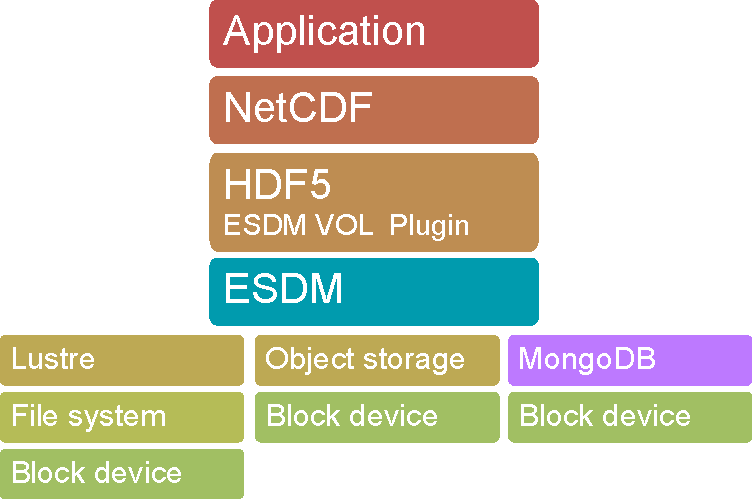
\includegraphics[width=0.5\columnwidth]{figures/layers-esdm}
    \caption{A typical I/O-stack with the ESD middleware}
    \label{fig:architecture-esd-layering}
\end{figure}

\begin{figure}[bp]
    \centering
    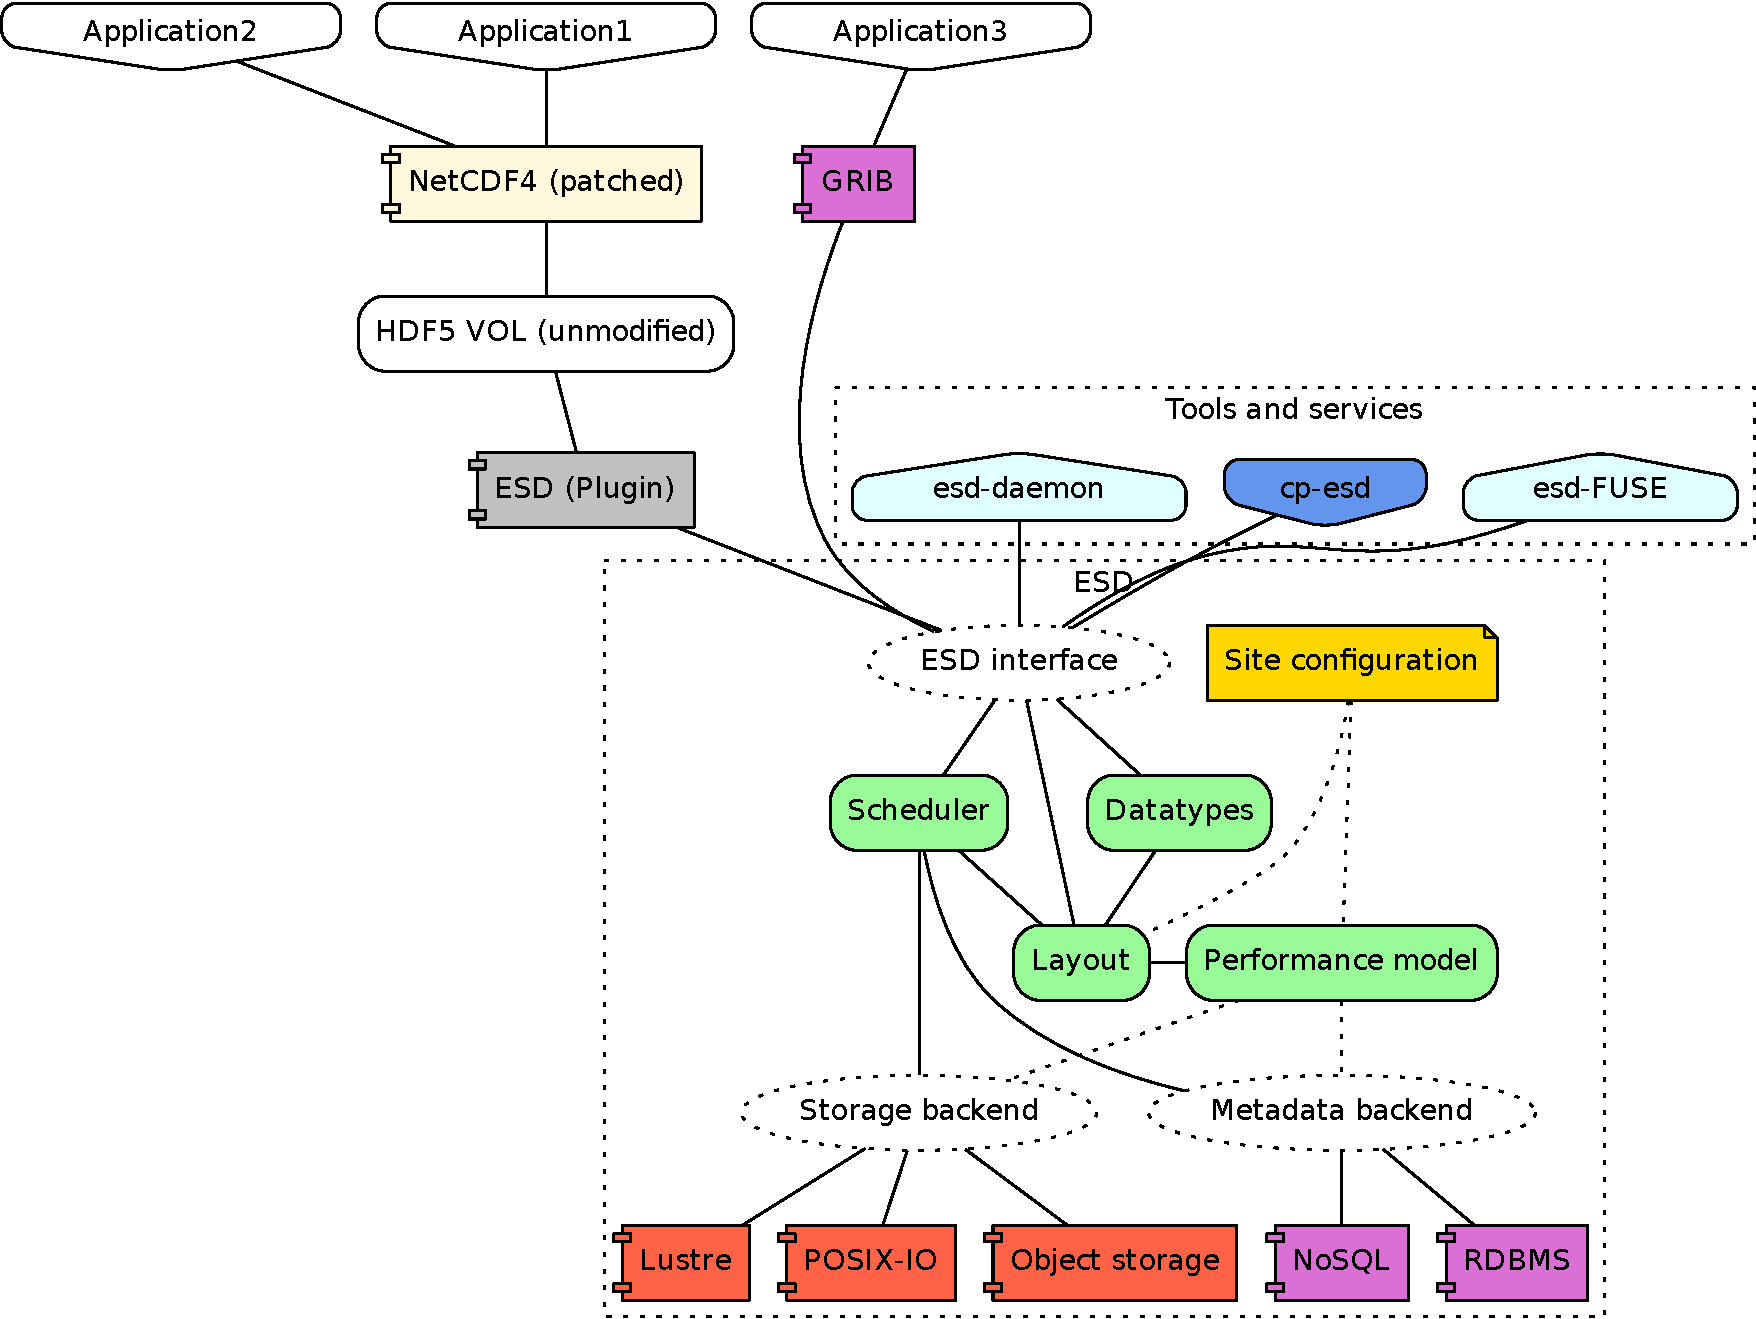
\includegraphics[width=0.98\columnwidth]{figures/architecture-backend-src.pdf}
    \caption{Overview of the ESD architecture, relevant components and relationship to application and storage systems.}
    \label{fig:architecture}
\end{figure}

A typical I/O-stack for an application using ESDM is shown in \Cref{fig:architecture-esd-layering}.
I/O of an existing application using the NetCDF (or HDF5) interface is processed by the ESDM plugin of HDF5 which may decide to store data on one of the available
storage backends such as Lustre or Object storage.
Metadata may be stored in one of the supported metadata plugins.
The user does not have to make decisions regarding the storage or metadata backends to be used; this decision is made by the middleware.

\bigskip


Details of the ESDM architecture is given in \Cref{fig:architecture}.
It provides more details about how ESDM is embedded into the existing software landscape and its high-level components:

\paragraph{Applications}
Use existing storage interfaces such as NetCDF4, GRIB or they may use the ESD interface.

\paragraph{Job scheduler}
The job scheduler assigns supercomputer resources to jobs.
It may use the ESD interface to inform about future activity and staged/unstaged data.


\paragraph{Middleware libraries} are adjusted to be layered on top of the ESD interface.


%%%%%%%%%%%%%%%%%%%%%%%%%%%%%%%%%%%%%%%%%%%%%%%%%%%%%%%%%%%%%%%%%%%%%%%%%%%%%%%
\paragraph{ESD Interface}
This represents the API exposed to other libraries and users.
The API is independent of the specific I/O backend used to store the data and supports structured queries to perform complex data selections in the variables.
The API is able to support the complex workflows of future applications.

%%%%%%%%%%%%%%%%%%%%%%%%%%%%%%%%%%%%%%%%%%%%%%%%%%%%%%%%%%%%%%%%%%%%%%%%%%%%%%%
\paragraph{Data types}
The data type component provides native data types that can be used by users or other libraries to describe data points inside variables.
We follow the approach pursued by the MPI and HDF5 libraries, that is, we provide a set of native data types and a basic set of data type constructors that can be used to build custom derived data types.

%%%%%%%%%%%%%%%%%%%%%%%%%%%%%%%%%%%%%%%%%%%%%%%%%%%%%%%%%%%%%%%%%%%%%%%%%%%%%%%
\paragraph{Layout}
The layout component allows the middleware to store pieces of data on different backends depending on specific site configuration contained in the performance model.
The layout component, in this case, takes responsibility for generating additional technical metadata describing data placement and for storing it in the appropriate metadata backend (i.e. MongoDB).
A more detailed description of what is technical metadata is given in the rest of this section.

\paragraph{Performance model}
This model predicts performance for data access using a site-specific configuration that describes the characteristics of available hardware technology.
It is used by the layout component to make decisions of the data placement.

\paragraph{Scheduler}
The scheduler queues asynchronous calls from the API and processes them.
It dispatches calls to storage and metadata backends and uses the layout component to identify the beneficial placement of data.

\paragraph{Metadata backend}
Responsible for storing all technical and scientific relevant metadata providing efficient access and manipulation.

\paragraph{Storage backend}
These backends are responsible for transforming ESD objects and data structures to storage-technology-specific representations.

\paragraph{Tools and services}
On top of ESDM several userspace tools are provided, a few examples are:
The FUSE client provides backwards POSIX compatibility with existing applications.
The daemon checks the consistency and integrity of the data managed by ESDM, potentially triggering actions to clean up and replicate data.
The copy tool allows importing and exporting data from ESD to existing storage infrastructure.
It also serves as a blueprint to embed its capabilities into higher-level tools such as GridFTP.

%%%%%%%%%%%%%%%%%%%%%%%%%%%%%%%%%%%%%%%%%%%%%%%%%%%%%%%%%%%%%%%%%%%%%%%%%%%%%%%%%%%%%%%%%%
\chapter{Logical View: Data Model}
\label{sec: viewpoints/logical/data model}

While data types introduced by computer architectures and software libraries are important for the data model, they are discussed separately in \Cref{sec: viewpoints/logical/data types}.

The data model of a system organises elements of data, standardises how they represent data entities and how users can interact with the data.
The model can be split into three layers:
\begin{enumerate}
    \item The \textbf{conceptual data model} describes the entities and the semantics of the domain. They are represented by the data model and the typical operations to manipulate the data.
    In our case, the scientific domain is NWP/climate.
    \item The \textbf{logical data model} describes the abstraction level provided by the system, how domain entities are mapped to objects provided by the system\footnote{A entity of the domain model such as a car could be mapped to one or several objects.}, and the supported operations for accessing and manipulating these objects are defined.
    Importantly, the \textbf{logical data model} defines the semantics when using the operations to access and manipulate the system objects.
    For example, a system object of a relational model is a table -- representing attributes of a set of objects -- and a row of a table representing attributes of a single object.
    \item The physical data model describes how the logical entities are finally mapped to objects/files/regions on available hardware.
    The physical data model is partly covered by the backends of ESDM. Therefore, the descriptions will stop at that abstraction level.
\end{enumerate}

\section{Conceptual Data Model}
\label{subsec: conceptual data model}

Our conceptual data model is aligned with the needs of domain scientists from climate and weather. It reuses and extends from concepts introduced in a data model proposed for the Climate and Forecasting conventions for NetCDF data\footnote {\url{ "A CF Data Model and Implementation", Hassel et al., 2017, GMD submitted}}.

\paragraph{Motivation from climate}



The ESDM needs to store, identify and manipulate data variables,  $V$, containing scientific data from the (continuous) real or model world, discretised within a "sampling" domain $d$, that is
\[V=V(d)\]
where $V$ may be air temperature, for instance. The domain $d$ describes the location for each value of $V$, and is a function of its independent dimensions, for instance
\[d = d(Z(z), Y(y), X(x)))\]
where $d$ is a three-dimensional domain described by axes of height, latitude, and longitude, sampled at coordinates found from the complete set of samples $Z(z), Y(y), X(x)$.
Each set of coordinates $x,y,z$  together specifies a location in the atmosphere at which $V$ is specified.



The full dimensionality of the variable may exceed the number of dimensions needed to store it --- for example, if $V$ is air-temperature at 1.5m, then $V$ may be sampled (and stored) in multiple 2-dimensional $x,y$ arrays, with each additional array representing a different time step.
In this case, some extra dimensions may be stored in the metadata accompanying the scientific data.



Sampling may be regularly spaced along one or more of the dimensions, in which case the coordinates (e.g., $x$) of the samples can be found algorithmically from the dimensions (e.g., $X$), and we describe the coordinate-grid as "structured" in those dimensions. Still, they can also be irregularly spaced, and their individual positions may need to be stored, in which case we describe the grid as "unstructured" in those dimensions.
With an unstructured grid, it is not possible to fully understand the domain distribution of $V$ unless all the coordinates are themselves stored as variables (e.g., $Z(z)$ is itself a variable defined at coordinates over a 1-dimensional domain spanning the height dimension).  A coordinate grid may be structured in one set of dimensions and unstructured in another.

\paragraph{}The values of $V$ at the coordinate positions may represent a value at that point, or be representative of an area, volume or face of a cell defined in one or more of the dimensions.

\paragraph{}In summary then, the conceptual (or scientific) data model consists of the following key entities:

\paragraph {Variable:} A variable, $V$, defines a set of data representing a discrete (generally scalar) quantity discretised within a ``sampling'' domain, $d$.  It is accompanied by

\paragraph {Metadata:} which will include at the minimum, a name, but may also include units, and information about additional dimensionality, directly (e.g. via a key, value pair such as that necessary to expose $z=1.5m$ for the air temperature at 1.5m) or indirectly (e.g. via pointers to other generic coordinate variables which describe the sampled domain).   There may also be a dictionary of additional metadata which may or may not conform to an external semantic convention or standard.  Such metadata could include information about the tool used to observe or simulate the specific variable.  Additional metadata is also required for all the other entities described below.

\paragraph{Dimension:} The sampling domain $d$ is defined by Dimensions which also defines a coordinate axis. Dimensions will include metadata, which have to include at a minimum a name (e.g. height, time). Still, they may also include information about directionality, units (e.g. degrees, months, days-since-a-particular-time-using-a-particular-calendar), or details of how to construct an algorithm to find the actual sampling coordinates, perhaps using a well-known algorithm such as an ISO 8601 time.

\paragraph{Coordinate:} Coordinates are the set of values at which data is sampled along any given dimension. They may be
explicitly defined by indexing into a coordinate variable, or implicitly defined by an algorithm. When we talk about the coordinates, it is usually clear if we mean the N-dimensional coordinate to address data in a given variable or if we just mean the (1D) coordinate along one dimension.


\paragraph{Cell:} The data values are known at points, which may or may not represent a cell. Such cells are N-dimensional shapes where the dimensionality may or may not fully encompass the dimensionality of the domain.
N-dimensional shapes can be implicitly defined in which case the Cartesian product of all dimensional coordinates forms the data "cube" of the cell. Still, they can also be explicitly defined, either by providing bounds on the coordinate variables (via metadata) or by introducing a new variable which explicitly defines the functional boundaries of the cell (as might happen in a finite element unstructured grid).


\paragraph{Dataset:} Variables can be aggregated into datasets. A dataset contains multiple variables that logically belong together, and should be associated with metadata describing the reason for the aggregation.  Variables must have unique names within a dataset.



Our conceptual model assumes that all variables are scalars, but clearly to make use of these scalars requires more complex interpretation.

\paragraph{Data type:}
which defines the types of values that are valid and the operations that can be conducted.
While we are mostly dealing with scalars, they may not be amenable to interpretation as simple numbers.
For example, a variable may be storing an integer which points into a taxonomy of categories of land-surface-types.
More complex structures could include complex data types such as vectors, compressed ensemble values, or structures within this system, provided such interpretation is handled outside of the ESDM and documented in metadata.  This allows us to limit ourselves to simple data types plus arbitrary length blocks of bits.

\paragraph{Operators:} Define the manipulations possible on the conceptual entities. The simplest operators will include creation, read, update and delete applied to an entity as a whole, or to a subset, however even these simple operators will come with constraints, for example, it should not be possible to delete a coordinate variable without deleting the parent variable as well. There will need to be a separation of concerns between operators which can be handled  \textit{within} the ESDM subsystem and those that require external logic. Operators which might require external logic include subsetting --- it will be seen that the ESDM will support simple subsetting using simple coordinates ---  but complex subsets such as finding a region in real space from dimensions spanned using an algorithm or coordinate variable, may require knowledge of how such algorithms or variables are specified.
Such knowledge is embedded in conventions such as the CF NetCDF conventions, and this knowledge could only be provided to the ESDM via appropriate operator plugins.

%\begin{figure}[b]
%    \centering
%    \includegraphics[width=5cm]{figures/data-model-variable}
%    \caption{Illustration of a 2D variable}
%    \label{fig:domainEntities}
%\end{figure}
% If we really want a figure, I've got a better one (BNL)



Whatever the sampling regime and dimensionality, values of a variable $V$ will be laid out in storage. In the next section (\ref{subsec-ldm}), we present the logical data model associated with the storage, before presenting a mapping of the conceptual data model to storage in section \ref{subsec-mapping}).


\section{Logical Data Model}
\label {subsec-ldm}

The logical data model describes how data is represented inside ESDM, the operations to interact with the data and their semantics. There are four first-class entities in the ESDM logical data model: \textbf{variable}s, \textbf{fragment}s, \textbf{container}s, and \textbf{metadata}. ESDM entities may be linked by ESDM \textbf{reference}s, and a key property which emerges from the use of references is that no ESDM entity instance may be deleted while references to it still exist. The use of reference counting will ensure this property as well as avoid dangling pointers.

\Cref{fig:data-model} gives an overview of the logical data model.



Each of these entities is now described, along with a list of supported operations:

\paragraph{Variable:} In the logical data model, the variable corresponds directly to a variable in the conceptual data model. Each element of the variable sampled across the dimensions contains data with a prescribed \textbf{DataType}.
Variables are associated with both \textbf{Scientific Metadata} and \textbf{Technical Metadata}. Variables are partitioned into \textbf{fragments} each of which can be stored on one or more "storage backend".
A variable definition includes internal information about the domain (bounding box in some coordinate system)  and dimensionality (size and shape), while the detailed information about which coordinate variables are needed to span the dimensions and how they are defined is held in the technical metadata.  Similarly, where a variable is itself a coordinate variable, a link to the parent variable for which it is used is held in the technical metadata.
The ESDM will not allow any attempt to delete a variable to succeed while any such references exist (see references).
A key part of the variable definition is the list of fragments associated with it, and if possible, how they are organised to span the domain.
Users may choose to submit code pieces that are then run within the I/O-path (not part within ESiWACE implementation), such an operation covers the typical filter, map and reduce operations of the data flow programming paradigm.

Fragments are created by the backend while appending/modifying data to a variable.

\textbf{Operations:}
\begin{itemize}
    \item Variables can be created and deleted.
    \item Fragments of data can be attached and deleted.
    \item Fragments can be repartitioned and reshuffled.
    \item Integrity can be checked.
    \item Data can be read, appended or modified those operations will be translated to the responsible fragments.
    \item Metadata can be atomically attached to a variable or modified.
    \item A variable can be sealed to make it immutable for all subsequent modifications.
    \item Process data of the variable somewhere in the I/O-path.
\end{itemize}

\paragraph{Fragment:}  A fragment is a piece (subdomain) of a variable. The ESDM expects to handle fragments as atomic entities, that is, only one process can write a fragment through the ESDM, and the ESDM will write fragments as atomic entities to storage backends.
The backends are free to further partition these fragments as is appropriate, for example, by sharding using chunks as described in section \ref{subsec-mapping}.
However, the ESDM is free to replicate fragments or subsets of fragments and to choose which backend is appropriate for any given fragment.
This allows, for example, the ESDM to split a variable into fragments, some of which are on stored on a parallel file system, while others are placed in object storage.

\textbf{Operations:}
\begin{itemize}
    \item Data of fragments can be read, appended or modified.
    \item Integrity of the fragment can be checked.
    \item Process data of the variable somewhere in the I/O-path.
\end{itemize}
%\todo{Resolve question on slack: \url{https://esiwace.slack.com/archives/C2T7KDRGC/p1496396797771552}}

\paragraph{Container:} A container is a virtual entity providing views on collections of variables, allowing multiple different datasets (as defined in the conceptual model) to be realised over the variables visible to the ESDM.  Each container provides a hierarchical namespace holding references to one or multiple variables together with metadata. Variables cannot be deleted while they are referenced by a container.  The use of these dynamic containers provides support for much more flexible organisation of data than provided by a regular file system semantics --- and efficiently support high-level applications such as the Data Reference Syntax\footnote{Taylor et al. (2012): CMIP5 Data Reference Syntax (DRS) and
Controlled Vocabularies.}.

A container provides the ESDM storage abstraction which is analogous to an external file. Because many scientific metadata conventions are based on semantic structures which span variables within a file in ways that may be opaque to the ESDM without the use of a plugin, the use of a container can indicate to the ESDM that these variables are linked even though the ESDM does not understand why, and so they cannot be independently deleted.
When entire files in NetCDF format are ingested into the ESDM, the respective importing tool must create a container to ensure such linking properties are not lost.

\textbf{Operations:}
\begin{itemize}
    \item Creation and deletion of containers.
    \item Creation and deletion of names in the hierarchical name space; the creation of links to an existing variable.
    \item Attaching and modification of metadata.
    \item Integrity can be checked.
\end{itemize}

\paragraph{Metadata:} can be associated with all the other first-class entities (variables, fragments, and containers). Such metadata is split into internal ESDM technical metadata and external user-supplied semantic metadata.
%A future version of the ESDM will support the internal exploitation of external metadata via plugins. Still, this version of the ESDM will treat external metadata as atomic and opaque, and simply serialise and store/replace/delete any such metadata. The internal metadata ...
%\todo {There needs to be a formal description of internal metadata}
Technical metadata covers, for example, permissions, information about data location and timestamps.
A backend will be able to add its own metadata to provide the information to look up the data for the fragment from the storage backend managed by it.
Metadata by itself is treated as a normal ESDM variable but linked to the variable of choice.
The implementation may embed (simple) metadata into fragments of original data (see Reference).

\textbf{Operations:}
\begin{itemize}
    \item Uses can create, read, or delete arbitrary scientific metadata onto variables and containers.
    A future version of the ESDM may support user scientific metadata for fragments.
    \item Container level metadata is generally not directly associated with variables but may be retrieved via following references from variables to containers.
    \item Queries allow to search for arbitrary metadata, e.g., for objects that have (\texttt{experiment=X, model=Y, time=yesterday})  returning the variables and containers in a list that match.
    This enables to locate scientific data in any arbitrary namespace.
\end{itemize}

\paragraph{Reference}
A reference is a link between entities and can be used in many places, references can be embedded instead of real data of these logical objects.
For example, dimensions inside a variable can be references. Also, a container typically uses references to variables.

\textbf{Operations:}
\begin{itemize}
    \item A reference can be created from existing logical entities or removed.
\end{itemize}


%\paragraph{Set}
%A set contains objects but only one object.




\begin{figure}
    \centering
    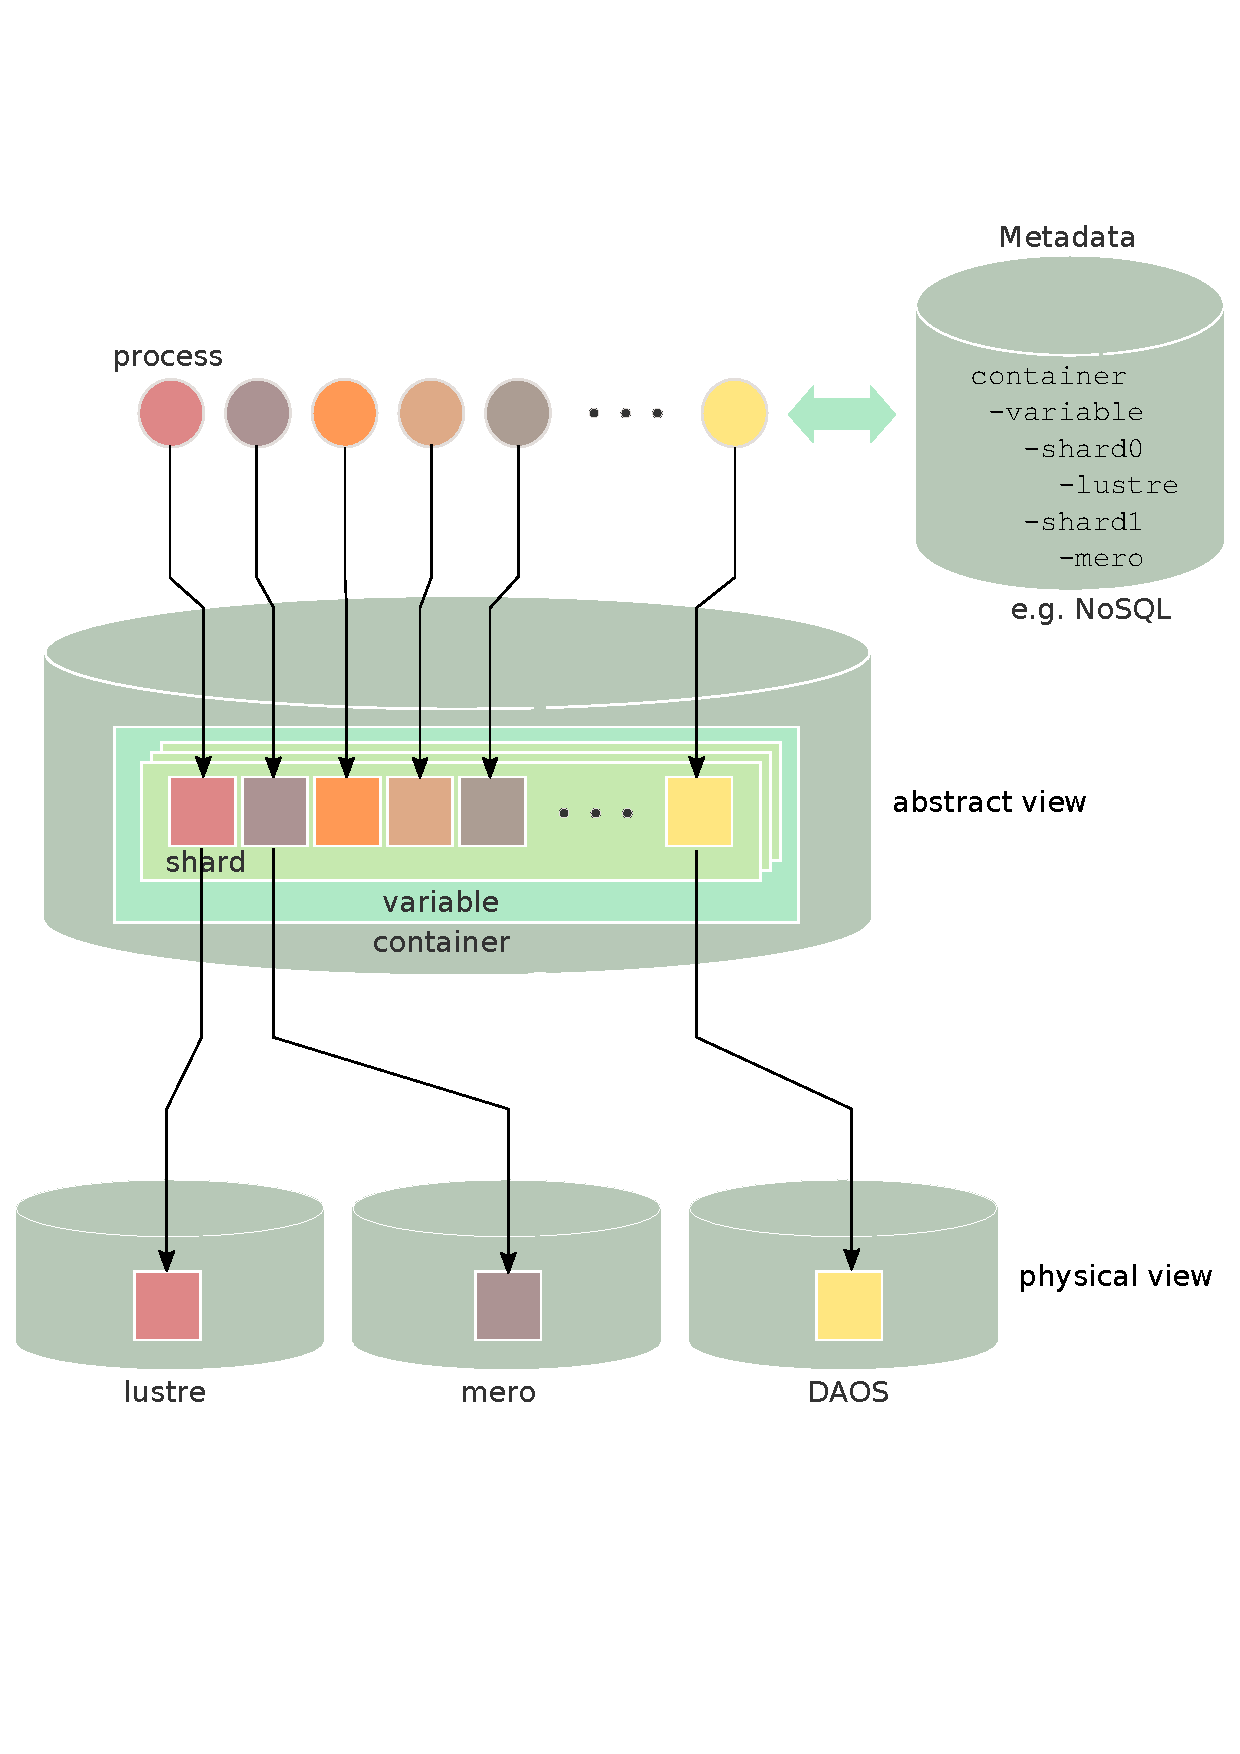
\includegraphics[width=0.5\textwidth]{data-model}
    \caption{Logical Data Model}
    \label{fig:data-model}
\end{figure}

\paragraph{Namespace}

ESDM does not offer a simple hierarchical namespace for the files.
It provides the elementary functions to navigate data: teleportation and orientation in the following fashion:
Queries about semantical data properties (e.g., \texttt{experiment=myExperiment, model=myModel, date=yesterday}) can be performed returning a list of matching files with their respective metadata.
Iterating the list (orientation) is similar to listing a directory in a file system.

Note that this reduces the burden to define a hierarchical namespace and for data sharing services based on scientific metadata.
An input/output container for an application can be assembled on the fly by using queries and name the resulting entities.
As a container provides a hierarchical namespace,
by harnessing this capability one can search for relevant variables and map them into the local file system tree, accessing these variables as if they would be, for example, NetCDF files.
By offering a FUSE client, this feature also enables backwards compatibility for legacy POSIX applications.



\section{Relationships between the Conceptual and Logical Data Model}
\label{subsec-mapping}

The conceptual logical data models are described above and summarised in \Cref{fig:cdm_ldm}.
These UML and this version of the architecture do not fully deal with the issues around coordinate systems which are not described by simple monotonic coordinate arrays, for which simple bounding boxes can be constructed.

As noted above, to fully exploit more complicated coordinate systems it will be necessary to describe those coordinate systems more fully in the scientific metadata (LDM\_Sci\_Metadata) and potentially provide a plugin to the system to handle them.
This notion is shown in the UML by virtue of the optional use of a named plugin to be identified in the scientific metadata, but the details of how that will work have been postponed to the prototype development.

\begin{figure}
    \centering
    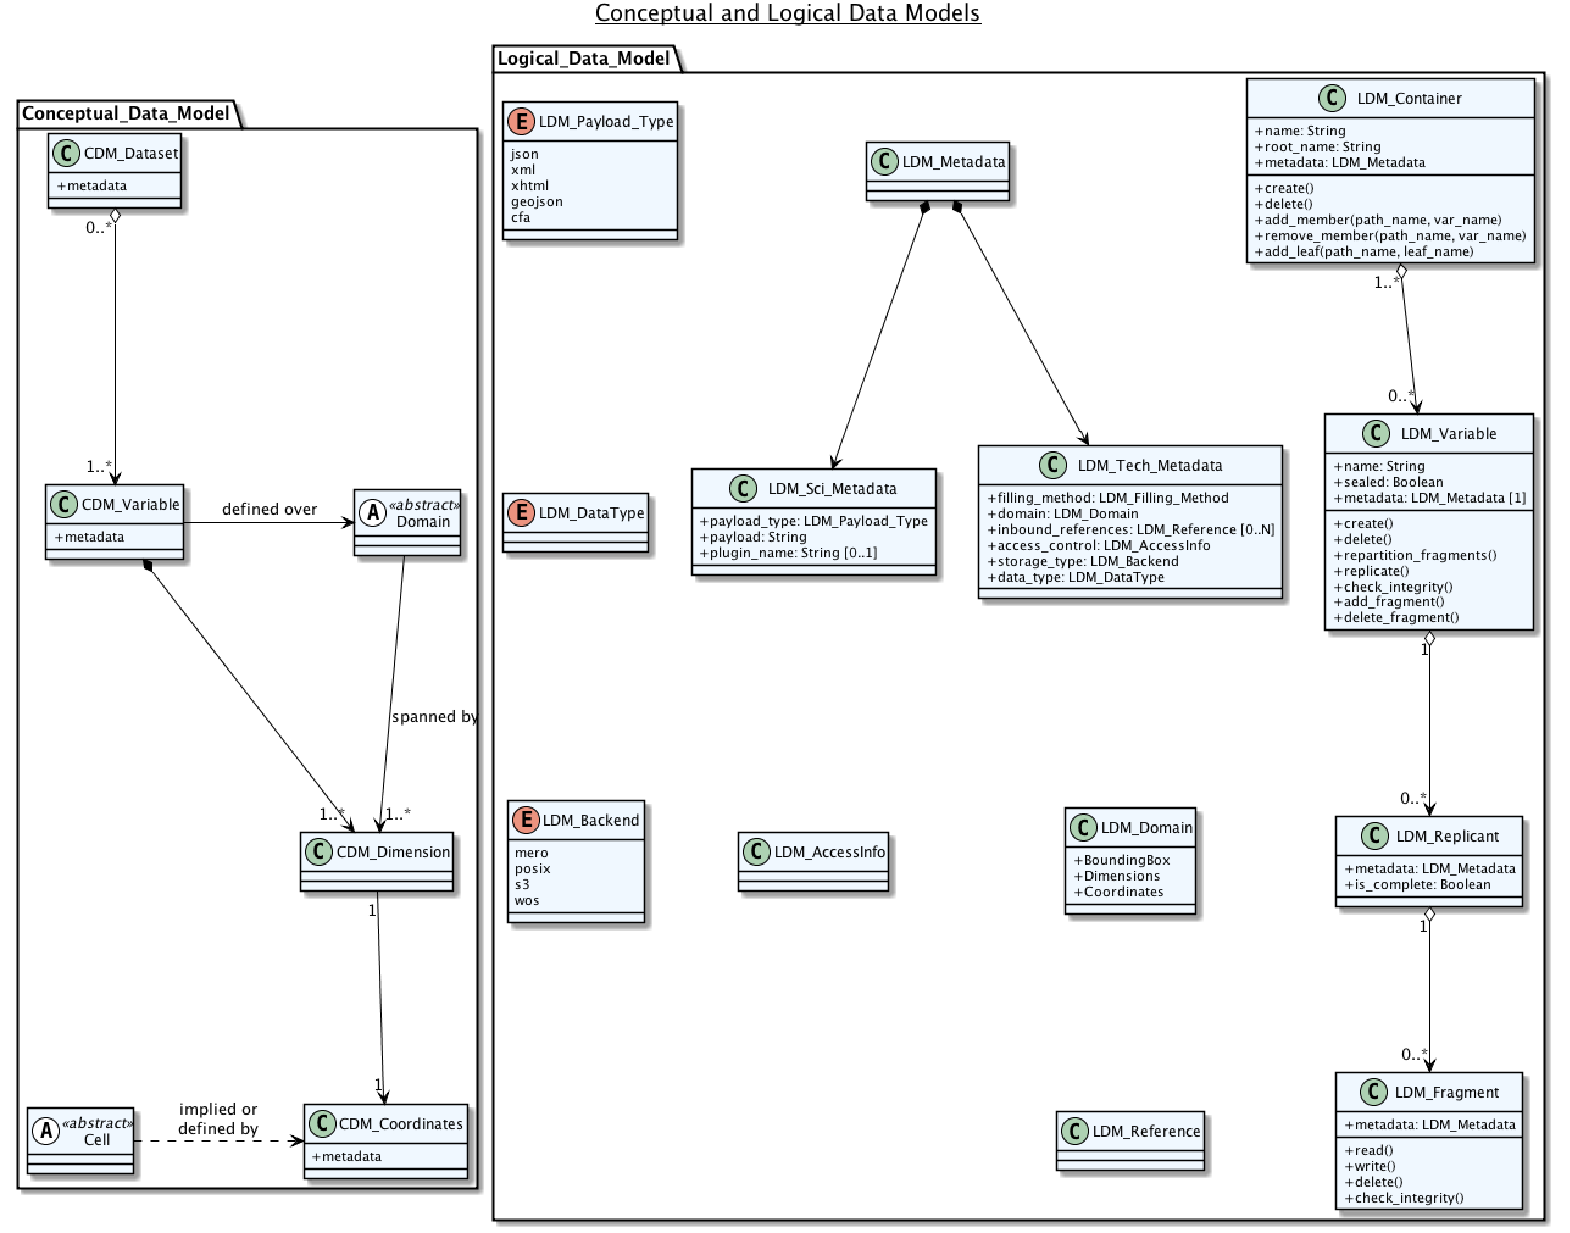
\includegraphics[width=\textwidth]{figures/cdm_ldm}
    \caption{A non-normative UML version of the conceptual and logical data models.
    The figure includes example for the operators of the invidiual logical operations.
    These UML are expected to be updated as the system is developed.  See also figure \ref{fig:dm_map}.}
    \label{fig:cdm_ldm}
\end{figure}

The key high-level entities are the conceptual container, variable, and domain, which have a direct correspondence in the logical
data model (see \Cref{fig:dm_map}). However, it is important to recognise that these are not isomorphic relationships. For example,
the concept of a domain of a variable in the conceptual model is expanded in the logical data model to include sub-domains associated
with fragments. Still, the same class is used for both usages (LDM\_Domain for both variable domain and fragment sub-domain).

\begin{figure}
    \centering
    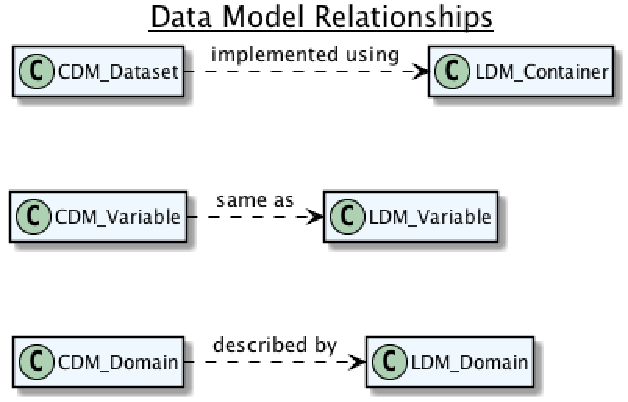
\includegraphics[scale=0.6]{figures/cdm_cdm}
    \caption{Key relationships between conceptual and logical data models.}
    \label{fig:dm_map}
\end{figure}

\section{Data types}
\label{sec: viewpoints/logical/data types}

The ESD middleware is specifically designed for weather and climate applications.
These applications usually use GRIB and NetCDF as data format to send and store
data. Nevertheless, the middleware should also be able to support other types of
applications that use arbitrary libraries to represent and store data.

The NetCDF and HDF5 libraries define their own atomic and basic data types and
then provide the APIs to build user-defined data types from these. Generally
speaking it makes sense to support a restricted number of most common data types
that application can use out of the box and offer the possibility of extending
these by means of additional APIs.

The support of native data types like H5T\_NATIVE\_INT or NC\_INT is driven by the necessity to decouple the internal representation of the data from the way data is ultimately stored.
Using native data types, data can be correctly reconstructed, passing from one representation to another.
Like other libraries, the ESD middleware will also support a restricted range of native data types and a series of dedicated APIs to build user-defined data types.

\medskip

ESDM will support various atomic data types, integers, floating points, with
different width, precision, endian and sign. The following table lists the
possible atomic data types:

\begin{center}
    \begin{tabular}{|c|c|}
        \hline
        type & description \\
        \hline
        ESDM\_T\_I8     & char                           \\
        ESDM\_T\_U8    & unsigned char                  \\
        ESDM\_T\_I16    & short (16bit)                  \\
        ESDM\_T\_U16   & unsigned short (16bit)         \\
        ESDM\_T\_I32      & integer (32bit)                \\
        ESDM\_T\_U32     & unsigned int (32bit)           \\
        ESDM\_T\_I64    & long long (64bit)              \\
        ESDM\_T\_U64   & unsigned long long (64bit)     \\
        ESDM\_T\_F16    & float (16bit)                  \\
        ESDM\_T\_F32    & float (32bit)                  \\
        ESDM\_T\_F64   & double (64bit)                 \\
        ESDM\_T\_F128 & long double (128bit)           \\
        ESDM\_T\_TIMESTAMP & Date and time stamp \\
        \hline
    \end{tabular}
\end{center}

User-defined complex data types include compound, variable-length array,
and array (fixed-length array).
The compound is similar to a struct in the C language.
It is an aggregation of members, which are atomic data types or another complex
data types.
The array has a fixed number of base data types, which are atomic data types
or other complex data types.
A variable-length array has a flexible length of base data types.

The definition of user-defined data types has to be stored on the backend. When reading data from datasets, these data types definition is retrieved from the backend
and parsed, and proper in-memory data structures and memories are allocated to
accommodate the expected data points.
Complex data types are encoded and stored on the backend in various formats according
to a different backend.
For example, for the Mero backend, this definition will be stored in a Key/Value pair in an index.
The data type is an integral part of the stored variable and fragment to allow the storage backend to understand the data and process it on demand (not part of the ESiWACE project).
\Cref{fig:data types} lists the required interfaces for the compound, array and key value based data structures.

\begin{figure}
    \centering
    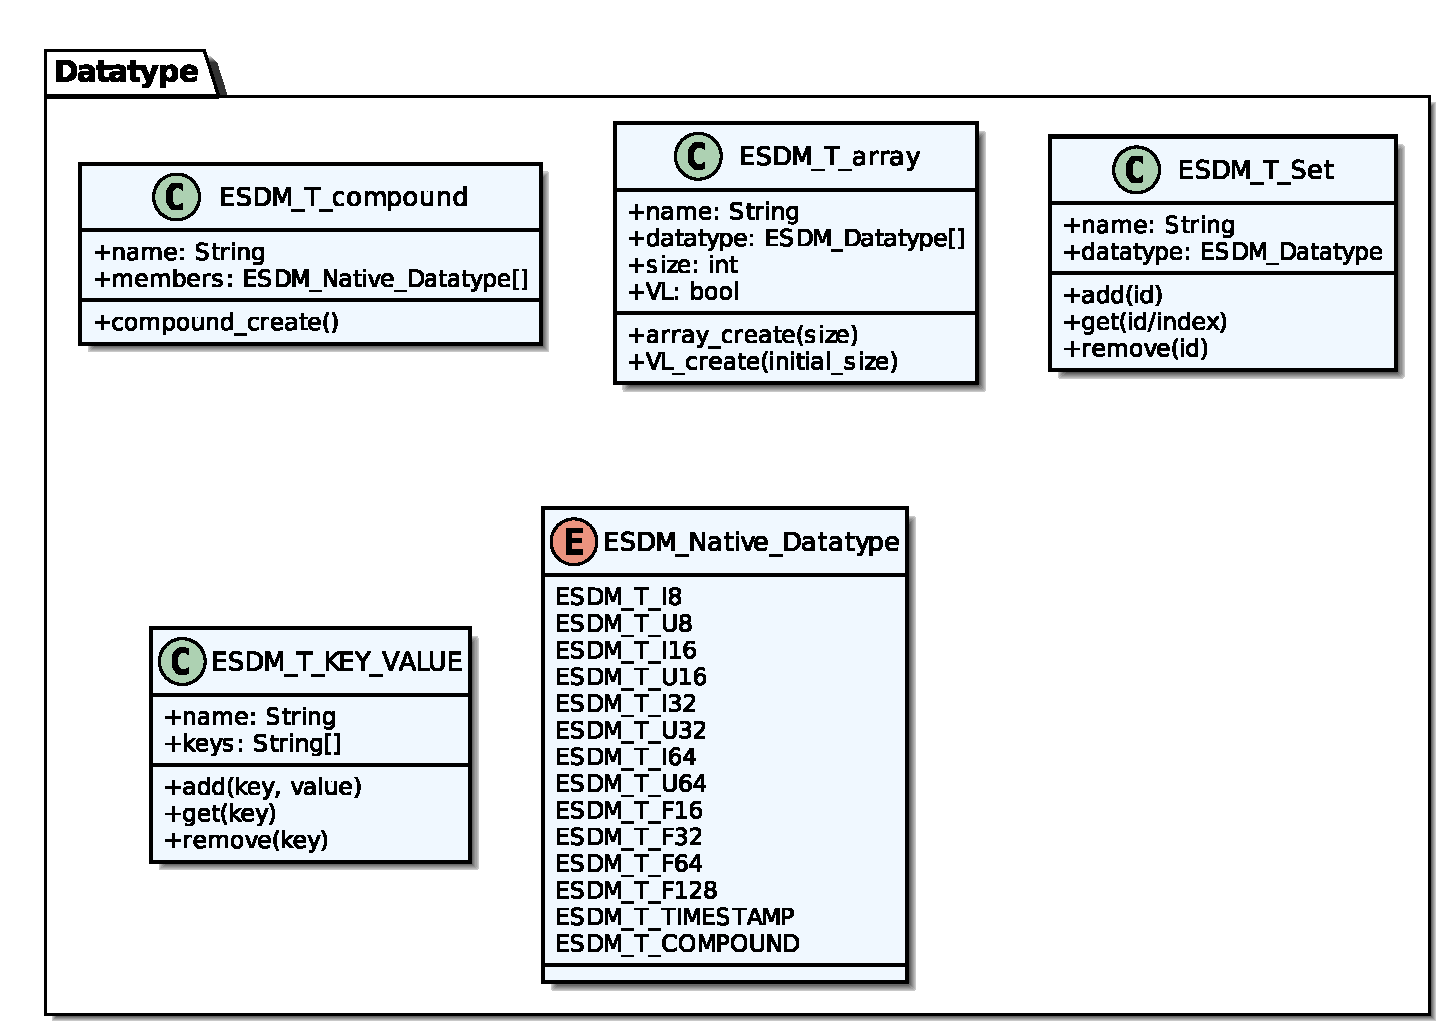
\includegraphics[width=0.9\textwidth]{figures/semantics-datatypes}
    \caption{Interfaces for the compound, array and key-value based data structures in relation to ESDM native data types.}
    \label{fig:data types}
\end{figure}

\chapter{NetCDF}

This section describes the implications in an existing parallel application that uses one of the supported interfaces such as NetCDF4/HDF5.
The semantics of the API calls will change slightly but typically in a way that is backwards compatible.

\section{Logical View}
\begin{figure}
    \centering
    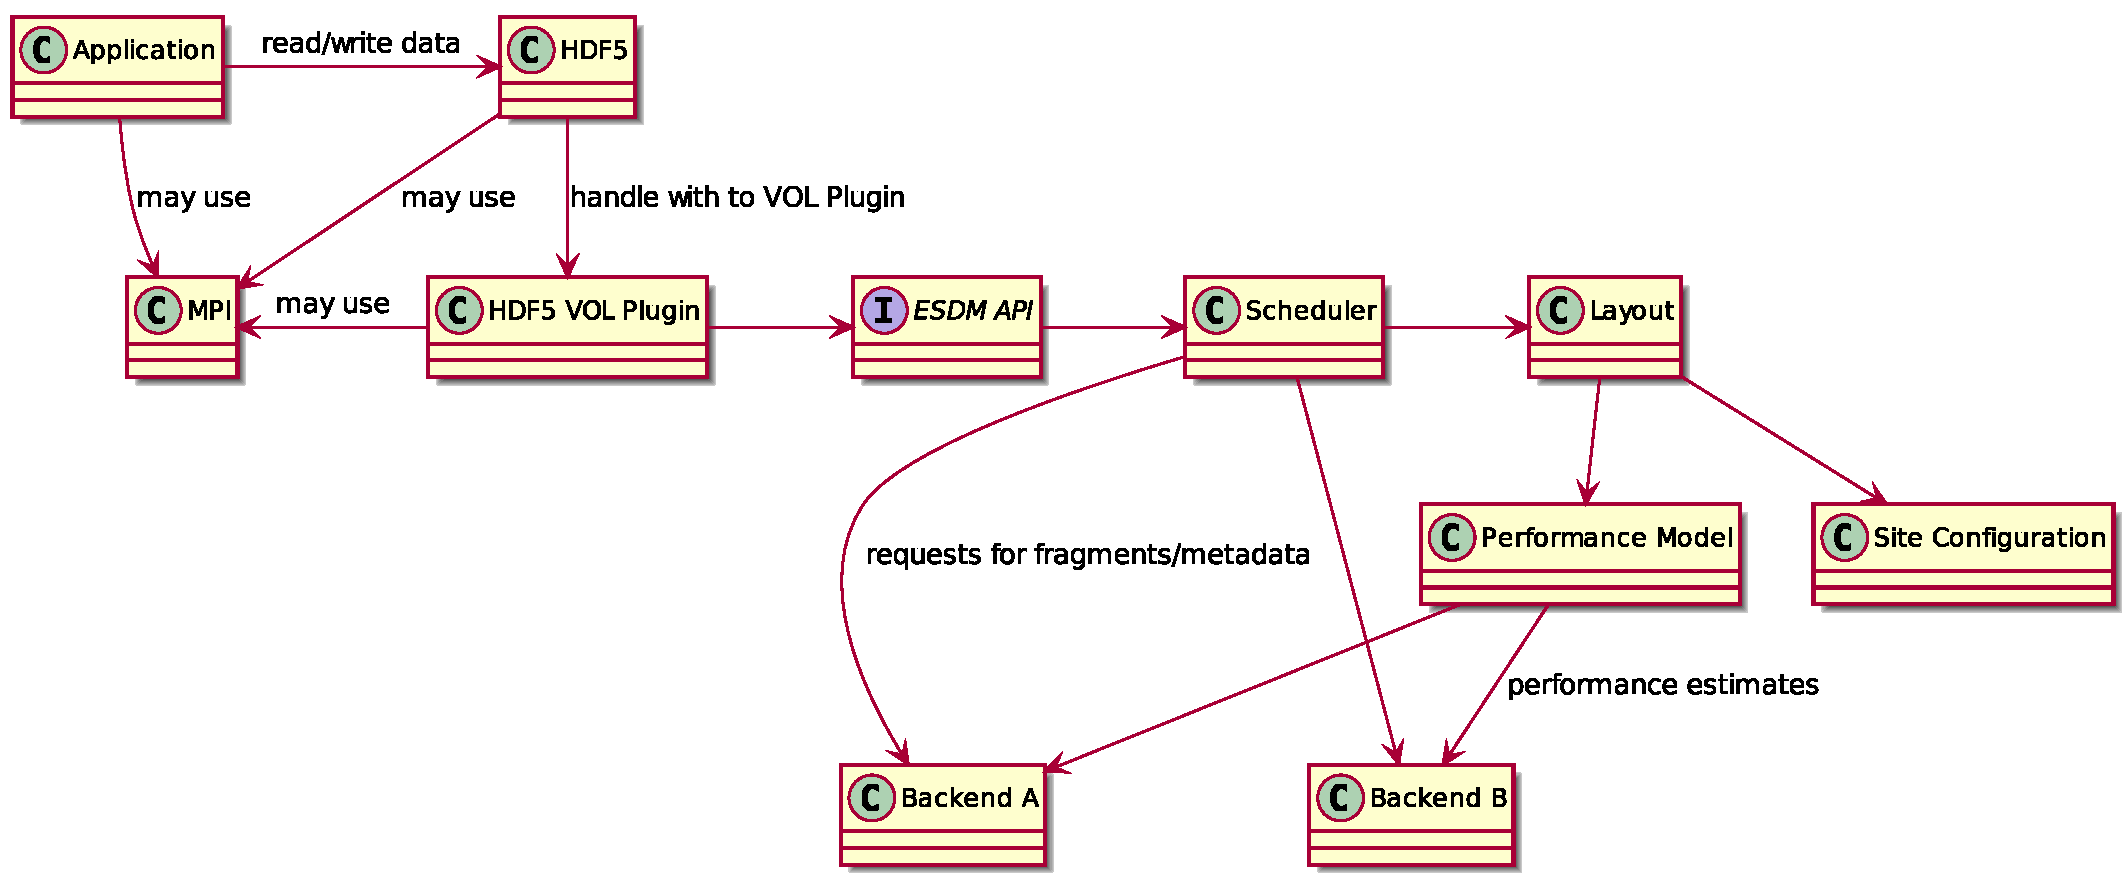
\includegraphics[width=\linewidth]{figures/logical}
    \caption{Logical view to the HDF+MPI plugin.}
    \label{fig:esdm hdf5 logical view}
\end{figure}

This subsection covers dealing with filenames, opening and closing of containers as well as concurrency semantics.
We assume an MPI parallelised application uses HDF5 with MPI support, e.g., parallel HDF5.
The component diagram in \Cref{fig:esdm hdf5 logical view} illustrates how an HDF5/NetCDF ESDM frontend would mediate between the ESDM and an application.
In addition, multiple processes using ESDM can coordinate using MPI, though only the ESDM component using MPI is the ESDM HDF5 VOL Plugin.

\subsection{Dealing with filenames}

Traditionally, when opening a file with NetCDF, the filename specifies the location, i.e., a URI where the data resides on a storage system.
We change the notion of the filename to be the descriptor for a virtual container (virtual container descriptor).
The virtual container can be composed of multiple URIs to integrate different variables into one virtual environment on the fly.
Thus, from the reader's perspective, it does not matter if data of a model is split into one or multiple physical files; upon read, all those files can be loaded together as if they would already exist in one logical file.
It is also possible to avoid the use of the metadata backend; by specifying the locations of the variables on existing storage media, they can be linked into a virtual container.
One restriction to this approach is the limitation of the length of filenames.
To avoid this limitation, we support a prefix to the filename: \texttt{esd-cfg:/} that leads to a simple JSON file that contains the actual definition of the container.

\subsection{Open}

Opening a container (as defined by the filename) in ESDM will trigger the master process within the communicator to retrieve the necessary metadata from ESDM and broadcast it to all participating processes.
Since the metadata is serializable to JSON, we can exchange the metadata easily.

\subsection{Concurrency semantics}

In general, the system is designed for parallel applications of which processes access data independently of each other.
Still, metadata of internal objects such as containers and variables should be managed and updated explicitly by a single process of the application.
That means, within one parallel (MPI) application, some kind of coordination must take place to allow the shared access to containers, variables and shards.
One correct implementation of this behaviour will be performed within the HDF5 VOL plugin.

Data sharing between independent applications is intended to happen after an epoch has been completed.
It is not allowed that multiple parallel applications write data to the same variable at the same time.
This is considered to be sufficient for most scenarios, e.g., a model produces some output; once the epoch completed, the produced data is post-processed.

\subsection{Close}

From the user perspective, closing a file that was opened in write mode, will make the content of the file visible in ESDM and durable for subsequent accesses.
Thus, it updates the metadata, for example, incrementing the epoch of the variables and containers modified and updating the reference counters.

\chapter{Metadata}

\section{Logical View}
\label{backend: mongo/logical}

\subsection{Metadata}

There are two methods to include metadata. Large metadata is included as a reference to another variable containing the data, and small metadata is embedded into the JSON of the MongoDB document.

Besides scientific metadata, the dynamic mapping of data to storage backends requires further metadata that must be managed.
To distinguish technical metadata from scientific metadata, an internal namespace is created.
Relevant technical metadata is shown in \Cref{tbl:additionalTechnicalMetadata} for shards, variables and containers, respectively.

Metadata can be optional (O) or mandatory (M), and either is created automatically or must be set manually via the APIs.
Automatic fields cannot be changed by the user.
Some of the data can be automatically inferred, if not set manually, but the manual setting may allow further optimisations.

Some of the metadata is used in several places. For example, information about the data lineage might be used to create several output variables.
In our initial implementation, the metadata is stored redundantly because:
1) it simplifies search; 2) it enables us to restore data on corrupted storage systems by reading the metadata; 3) it reduces contention and potentially false sharing of metadata.
An implementation might decide to reduce this by utilising normalised schemas.

References are the list of objects that are directly used by this object, e.g., other variables that are used to define the data further.

\begin{table}
    \begin{subtable}[t]{\textwidth}
        \begin{tabular}{llll}
            Metadata & Field & Creation & Description\\
            \hline
            Domain   & M & Auto & The subdomain this data covers from the variable\\
            Type     & M & Auto & The (potentially derived) data type of this shard\\
            Variable & M & Auto & The ID of the varitechnical-on-metadata.texable this data belongs to\\
            Storage  & M & Auto & The storage backend used and its options\\
            References & M & Auto & A list of objects that are referenced by this data\\
            Sealed   & M & Auto & A sealed shard is read-only\\
        \end{tabular}
        \caption{For a shard}
    \end{subtable}

    \begin{subtable}[t]{\textwidth}
        \begin{tabular}{llll}
            Metadata & Field & Creation & Description\\
            \hline
            Domain      & M & Manual & Describes the overall domain\\
            Type           & M & Manual & The (potentially derived) data type\\
            Info           & M & Manual & The scientific metadata of this document\\
            References  & M & Auto & A list of objects that are referenced by this data\\
            Permissions & M & Auto/Manual & The owner and permissions \\
            Shards      & M & Auto & The list of shard objects for this variable\\
            Sealed      & M & Auto & A sealed variable is read-only\\
        \end{tabular}
        \caption{For a variable}
    \end{subtable}


    \begin{subtable}[t]{\textwidth}
        \begin{tabular}{llll}
            Metadata & Field & Creation & Description\\
            \hline
            Owner    & O     & Manual   & The owner of this file view (see the permission model)\\
            Info     & O     & Manual   & Additional scientific metadata for this view\\
            Directory & O    & Manual   & Contains a mapping from names to variables\\
            Environment & O  & Automatic & Information about the application run\\
            Permissions & M & Auto/Manual & The owner and permissions \\
            References  & M & Auto & A list of objects that are referenced by this data.
        \end{tabular}
        \caption{For a container}
    \end{subtable}
    \caption{Excerpt of additional technical metadata}
    \label{tbl:additionalTechnicalMetadata}
\end{table}




%%%%%%%%%%%%%%%%%%%%%%%%%%%%%%%%%%%%%%%%%%%%%%%%%%%%%%%%%%%%%%%%%%%%%%%%%%%%%%%
\section{Mapping of metadata}

To illustrate the applied mapping, we use a subset of our NetCDF metadata described in \Cref{sec:netcdfDataMapping}.
The excerpt is given in \Cref{lst:NetCDF-data-map}.
The mapping of a single logical variable is exemplarily described in \Cref{lst:NetCDF-data-map}.


\begin{tcbcode}[label={lst:NetCDF-data-map}]{NetCDF metadata for one variable}
\begin{lstlisting}[upquote=true]
dimensions:
    longitude = 480 ;
    latitude = 241 ;
    time = UNLIMITED ; // (1096 currently)
variables:
    float longitude(longitude) ;
        longitude:units = "degrees_east" ;
        longitude:long_name = "longitude" ;
    float latitude(latitude) ;
        latitude:units = "degrees_north" ;
        latitude:long_name = "latitude" ;
    int time(time) ;
        time:units = "hours since 1900-01-01 00:00:0.0" ;
        time:long_name = "time" ;
        time:calendar = "gregorian" ;
    short sund(time, latitude, longitude) ;
        sund:scale_factor = 0.659209863732776 ;
        sund:add_offset = 21599.6703950681 ;
        sund:_FillValue = -32767s ;
        sund:missing_value = -32767s ;
        sund:units = "s" ;
        sund:long_name = "Sunshine duration" ;

// global attributes:
        :Conventions = "CF-1.0" ;
        :history = "2015-06-03 08:02:17 GMT by grib_to_netcdf-1.13.1: grib_to_netcdf /data/data04/scratch/netcdf-atls14-a562cefde8a29a7288fa0b8b7f9413f7-lFD4z9.target -o /data/data04/scratch/netcdf-atls14-a562cefde8a29a7288fa0b8b7f9413f7-CyGl1B.nc -utime" ;
}
\end{lstlisting}
\end{tcbcode}

To simplify search and identify data clearly, data services such as the WDCC and CERA, that offer data to the community, request scientists to provide additional metadata.
Normally, such data is provided when the results of an experiment are ingested into such a database.
Example metadata is listed in \Cref{tbl:additionalMetadata}.
In existing databases, the listed metadata is split into several fields, e.g. an address and email for persons, for simplicity only a rough overview is given.
Instead of encoding the history as a simple text field, it could
indicate detailed steps, including the arguments for the commands and versions and transformations to reproduce the data.
This should include for each step, where and the time when it is performed, and the versions of software used.

It is easily imaginable that most of this information could be useful already when the data is created as it simplifies the search and data management on online storage.
Some of the data fields become only available after the initial data creation, e.g., the DOI.
Potentially the data must be updated/curated after the data is created.

\begin{table}
\begin{tabular}{ll}
Metadata & Description\\
\hline
Project & The scientific project during which the data is created \\
Institute & The institution which conducted the experiment\\
Person &  A natural person; could be a contact, running the experiment \\
Contact & Reference to person or consortium \\
DOI      & A document object identifier; useful for identifying a data publication\\
Topic     & Some information about the topic of the data / experiment \\
Experiment & Description of this particular experiment \\
History & A list with the history and transformations conducted with the data \\
\end{tabular}
\caption{Excerpt of additional scientific metadata}
\label{tbl:additionalMetadata}
\end{table}



\section{Example}

This example illustrates data of a predictive model could be stored on the system and the resulting metadata.
The dimensionality of the underlying grid is fixed.

The application uses the following information to drive the simulation:
\begin{itemize}
    \item Timerange: the simulated model time (from a starting datetime to the specified end)
    \item Longitude/Latitude: 1D data field with the coordinates [float]
    \item Temperature: Initial 2D field defined on (lon, lat)
\end{itemize}
A real model would use further parameters to estimate the temperature, but these are sufficient to demonstrate the concepts.
This information is either given as a parameter to the simulation or read from an input (container).
A mixture of both settings is possible.


The application produces the following output:
\begin{itemize}
    \item Longitude/Latitude: 1D data field with the coordinates [float]
    \item Model time: the current datatime for the simulation
    \item Temperature: 2D field defined on (lon, lat, time) [float], containing the precise temperature on the coordinates defined by lon and lat for the given timestep
    \item AvgTemp: 1D field defined on (time) [float]; contains the mean temperature for the given time
\end{itemize}

\subsection{Container}

Upon application startup, we create a new virtual container that provides links to the already existing input.
In \Cref{lst:mongoContainer}, the metadata for the container is shown after the application is started.
We assume it has used the APIs to provide the information (input, output, scientific metadata).
In this example, we explicitly define the objects used as input; it is possible to also define
the input as an already existing container.
It is also possible to define the input a priori if the objectIDs are known/looked up prior application run.
The intended output variables could be given with their rough sizes.
This would allow the scheduler to pre-stage the input and ensure that there is enough storage space available for the output.
The environment information is inferred to the info object but can be changed from the user.

\begin{tcbcode}[label={lst:mongoContainer}]{JSON document describing the container}
    \begin{lstlisting}[upquote=true]
    "_id" : ObjectId(".."),
    "directory" : {
        "input" : {
            "longitude" : ObjectId(".."),
            "latitude" : ObjectId(".."),
            "temperature" : ObjectId("..")
        },
        "output" {
            "temperature" : ObjectId(".."),
            "avgTemp" : ObjectId("..")
        }
    },
    "info" : { # This is the scientific metadata
        "model" : { "name" : "my model", "version" : "git ...4711" },
        "experiment" : {
            "tags"        : ["simulation", "poisson", "temperature"]
            "description" : "Trivial simulation of temperature using a poisson process"
        },
    },
    "environment" : {
        "date"  : datetime(2016, 12, 1),
        "system" : "mistral",
        "nodes" : ["m[1-1000]"]
    },
    "permissions" : {
        "UID"  : 1012,
        "GID"  : 400,
        "group" : "w", # allows read also
        "other" : "r"
    },
    "references" : {
        [ all links to used object IDs from input / output ]
    }
    \end{lstlisting}
\end{tcbcode}

\subsection{Variable}

The metadata for a single variable is build based on the information available in the container (such as permissions) and additional data provided by the user.
Indeed, part of the metadata is replicated between container and variable as this preserves information about the creation of the variable that will typically not change during the lifetime of the variable.

An example of the temperature variable is shown in \Cref{lst:mongotemperature}.
When describing the domain that is covered by the variable, there are three alternatives:
1) a reference to an existing variable is embedded, and the minimum / maximum value is provided.
This allows reusing descriptive information as data has to be stored only once. Min and max describe the multidimensional index of the subdomain in the variable that is actually referenced;
2) data becomes embedded in the file. This option is used when the size of the variable is small.
An advantage of option 2) is that searches for data with a certain property do not require to lookup information in additional metadata.

Similarly, information about the data lineage (history) can originally be inferred from the objects linked in the directory mapping.
In that case, the metadata of the referenced object must be copied, if the original object is removed.

3) A plugin for the interpretation and mapping of the coordinate system is used.
The plugin name must be stored and the respective parameters to identify the coordinates stored.


\begin{tcbcode}[label={lst:mongotemperature}]{JSON document for temperature}
    \begin{lstlisting}[upquote=true]
    "_id" : ObjectId("<TEMPID>"),
    "sealed" : true,
    "domain" : [
        "longitude" : [ "min" : 0, "max" : 359999, "reference" : ObjectId("..") ],
        "latitude" : [ "min" : 0, "max" : 179999, "reference" : ObjectId("..") ],
        "time" : [ datetime(...), datetime(...), ... ]
    ],
    "type" : "float",
    "info" : {
        "convention" : "CF-1.0",
        "name" : "temperature",
        "unit" : "K",
        "long description" : "This is the temperature",
        "experiment" : {
            "tags"        : ["simulation", "poisson", "temperature"]
            "description" : "Trivial simulation of temperature using a poisson process"
        },
        "model" : { "name" : "my model", "version" : "git ...4711" },
        "directory" : {
            "input" : {
                "longitude" : ObjectId("<LONID>"),
                "latitude" : ObjectId("<LATID>"),
                "temperature" : ObjectId("<TEMPID>")
            }
    },
    "environment" : {
        "date"    : datetime(2016, 12, 1),
        "system" : "mistral",
        "nodes"  : ["m[1-1000]"]
    },
    "history" : [
        ...
    ],

    "permissions" : {
        "UID"  : 1012,
        "GID"  : 400,
        "group" : "w", # allows read also
        "other" : "r"
    },
    "references" : {
        [ all links to used object IDs ]
    },
    "shards" : [
        ObjectId(<SHARD1 ID>),
        # For a sealed object, the domains of its shards can optionally be embedded:
        { "reference" : ObjectId(<SHARD2 ID>), "storage" : ... , "domain" },
        ObjectId(<SHARD3 ID>),
        ObjectId(<SHARD4 ID>)
    ]
    \end{lstlisting}
\end{tcbcode}

\subsection{Shards}

The variable is split into multiple shards; metadata for one of them is shown in \Cref{lst:mongotemperatureshard}.
Since we assume domain decomposition in the application, the longitude and latitude variables are now only partially stored in a shard.
In the example, we assume two processes create one shard each and the surface of the earth is partitioned into four non-overlapping rectangles.

\begin{tcbcode}[label={lst:mongotemperatureshard}]{JSON document for a shard of the temperature variable}
\begin{lstlisting}[upquote=true]
"_id" : ObjectId("<SHARD1 ID>"),
"sealed" : true,
"variable" : ObjectId("<TEMPID>"),
"type" : "float",
"domain" : {
    "longitude" : [ "min" : 0, "max" : 179999, "reference" : ObjectId("..") ],
    "latitude" : [ "min" : 0, "max" : 89999, "reference" : ObjectId("..") ],
    "time" : [ datetime(...), datetime(...), ... ]
},
"storage" : {
    "plugin" : "pfs",
    "options" : {
        "path" : "/mnt/lustre/testdir/file1",
    },
    "serialization" : "row-major"
},
"references : [
    ObjectId("<TEMPID>"),
    ObjectId(".."),
    ObjectId("..")
]
\end{lstlisting}
\end{tcbcode}

\end{comment}
